\chapter{Non-deterministic PI}

Pair-Interaction that Nasilowski proposed is deterministic, and it might be considered to be its advantage. 
The collision (usually) leads to the maximal change of the state, that minimizes the viscosity (as we previously discussed).
Moreover, it offers theoretical ground for using Gibbs distribution in derivation of macroscopic equations.

\bigskip

But let us explore following examples.
First, consider node with one standing particle.
\begin{figure}[h]
 \centering 
 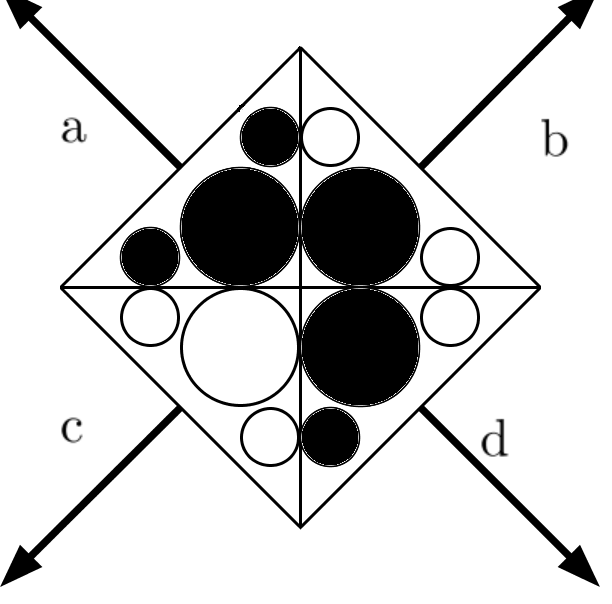
\includegraphics[width=0.22\textwidth]{../nonPInode/node_1}
 \label{transitions}
 \caption{Node before collision}
\end{figure}

By deterministic pair-interactions in X,Y and Z direction, it is always resolved into the state
\begin{figure}[h]
 \centering 
 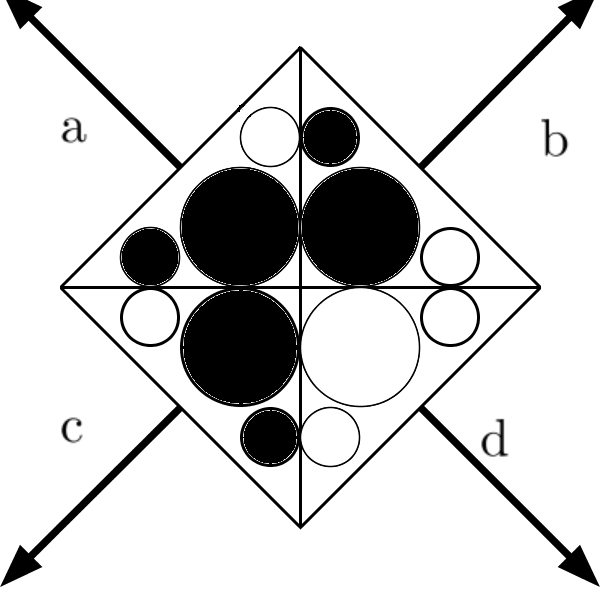
\includegraphics[width=0.22\textwidth]{../nonPInode/node_2}
 \label{transitions}
 \caption{Node after deterministic collision}
\end{figure}

But it is no better then

\begin{figure}[h]
 \centering 
 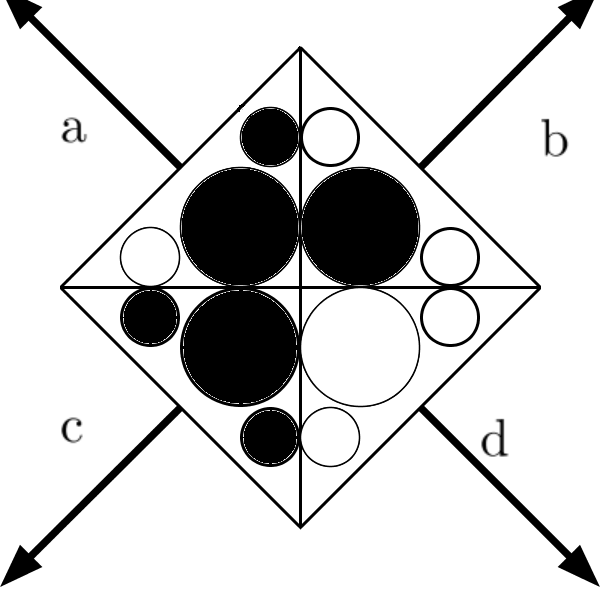
\includegraphics[width=0.22\textwidth]{../nonPInode/node_3}
 \label{transitions}
 \caption{Another acceptable state after collision}
\end{figure}

or any other state with one standing particle.

\bigskip
\newpage
Even better example is the node with two particles with momenta in X direction.
\begin{figure}[htbp]
 \centering 
 \includegraphics[width=0.28\textwidth]{../nonPInode/mom1}
 \label{transitions}
 \caption{Node before collision, and after deterministic collision}
\end{figure}

The deterministic collision do not change its state (pair interaction in Y direction, followed by pair interaction in Z direction leads to the same state for this particular example).

However, collision that would be non-deterministic (let's say that pair interaction happens with probability $1/2$) can lead to the following state
\begin{figure}[htbp]
 \centering 
 \includegraphics[width=0.28\textwidth]{../nonPInode/mom2}
 \label{transitions}
 \caption{Node after non-deterministic collision}
\end{figure}

where both particles gained additional momenta, one in Z, and other in -Z direction.
We could continue with the examples showing that deterministic PI do not realize all available states, even though some of them are more desirable. 

Also, by chosing one of the many available states by non-deterministic PI, we believe that statistical avareging might work faster and lead to better results when statistical properties of the flow are inspected.

\bigskip

On the other hand, non-deterministic model, has one obvious drawback. Generation of random numbers is costy process and significantly slows down the collisions (although it might be cheated, we prefer to try honest non-deterministic model, then we can optimize).

The non-deterministic automaton was achieved by simple modification of the collision algorithm.

\begin{lstlisting}
void Collision(Node***array, int X, int Y, int Z, int start)
{
	/* Rundom numbers are generated by Mersen-Twister pseudo-random generator */
	random_device rd;
	mt19937 rng(rd());
	
	/* As there are 12 pair interactions per one collision, we want to generate 12 random bits with uniform distribution */
	int upper = pow(2, 12);
	uniform_int_distribution<int> uni(0,upper - 1);
	
	int r;
	int x,y,z;

#pragma omp parallel for private (x,y,z)
	for (x = start; x < X; x+=2)
	{
		for(y = start; y < Y; y+=2)
		{
			for(z = start; z < Z; z+=2)
			{
					r =  = uni(rng);
					array[x][y][z] = collision(array[x][y][z], r);
			}
		}
	}
}

/*  Comparing to deterministic collision function, it has second parameter ran */
/* first 12 bi
Node collision(Node node, int ran)
{
	//mass
	unsigned char m = node.m;
	
	//momentum
    unsigned char *p = node.p;

	//d,u ... index for downer and upper momentum
	int d,u;
    
	// l, r ... left/right cell in the pair
	// ml, mr ... particle in left/right cell is present (mass-left, mass-right)
	// lu, ld, ru, rd ... momenta of particles (left-upper, left-downer, right-upper, right-downer)
	unsigned char l, r, ml, mr, lu, ld, ru, rd;

	// For first pair-interaction, first bit is set to one, other bits are zero
	int count = 1;
	for (int i = 0; i < 3; ++i)
	{
		d = (i+1) % 3;
		u = (i+2) % 3;
		for (int j = 0; j < 4; ++j)
		{
			/* If the ran has corresponding bit equal to 1, the pair-interaction go on, else it is skipped */
			if (!( ran &count))
			{
				count <<= 1;
				break;
			}
			count <<= 1;
			....
			....
			/* The rest of the function is not modified */
\end{lstlisting}

\section{Exploding cube}
To demonstrate the difference of deterministic and non-deterministic automaton in the crystal form, we simulated the "explosion of the cube". 

The simulations were performed on the lattice $240 \cross 240 \cross 240$ nodes for deterministic PI, and for the slower non-deterministic PI, size of the domain was $120 \cross 120 \cross 120$. Periodic boundary conditions were used.

Into the cube with the side of the length 3 times smaller then the lattice (hence the volume of the cube was $1/27$ of the lattice), we put particles into all available cells, with maximal momenta in all directions. Therefore, the total momentum of the particles is 0.

The evolution of the system for both versions of PI is to be seen on the following pictures.

\begin{figure}[h]
 \centering 
 \includegraphics[width=0.9\textwidth]{../kocka_utlm/velocity_0}
 \caption{Deterministic PI - time 0}
\end{figure}

\begin{figure}[h]
 \centering 
 \includegraphics[width=0.9\textwidth]{../kocka_utlm/velocity_6}

% \caption{Deterministic PI - time 6}
\end{figure}

\begin{figure}[h]
 \centering 
 \includegraphics[width=0.9\textwidth]{../kocka_utlm/velocity_12}
 \caption{Deterministic PI - time 12}
\end{figure}

\begin{figure}[h]
 \centering 
 \includegraphics[width=0.9\textwidth]{../kocka_utlm/velocity_36}
 \caption{Deterministic PI - time 36}
\end{figure}

\begin{figure}[h]
 \centering 
 \includegraphics[width=0.9\textwidth]{../kocka_utlm/velocity_84}
 \caption{Deterministic PI - time 84}
\end{figure}

\begin{figure}[h]
 \centering 
 \includegraphics[width=0.9\textwidth]{../kocka_utlm/velocity_102}
 \caption{Deterministic PI - time 102}
\end{figure}

\begin{figure}[h]
 \centering 
 \includegraphics[width=0.9\textwidth]{../kocka_utlm/velocity_126}
 \caption{Deterministic PI - time 126}
\end{figure}


\begin{figure}[h]
 \centering 
 \includegraphics[width=0.9\textwidth]{../kocka_utlm/velocity_162}
 \caption{Deterministic PI - time 162}
\end{figure}


\begin{figure}[h]
 \centering 
 \includegraphics[width=0.9\textwidth]{../kocka_utlm/velocity_174}
 \caption{Deterministic PI - time 174}
\end{figure}


\begin{figure}[h]
 \centering 
 \includegraphics[width=0.9\textwidth]{../kocka_utlm/velocity_198}
 \caption{Deterministic PI - time 198}
\end{figure}


\begin{figure}[h]
 \centering 
 \includegraphics[width=0.9\textwidth]{../kocka_utlm/velocity_234}
 \caption{Deterministic PI - time 234}
\end{figure}


\begin{figure}[h]
 \centering 
 \includegraphics[width=0.9\textwidth]{../kocka_utlm/velocity_282}
 \caption{Deterministic PI - time 282}
\end{figure}


\begin{figure}[h]
 \centering 
 \includegraphics[width=0.9\textwidth]{../kocka_utlm/velocity_312}
 \caption{Deterministic PI - time 312}
\end{figure}


\begin{figure}[h]
 \centering 
 \includegraphics[width=0.9\textwidth]{../kocka_utlm/velocity_324}
 \caption{Deterministic PI - time 324}
\end{figure}




\begin{figure}[h]
 \centering 
 \includegraphics[width=0.9\textwidth]{../kocka_utlm_1/velocity_6}
 \caption{Non-deterministic PI - time 6}
\end{figure}


\begin{figure}[h]
 \centering 
 \includegraphics[width=0.9\textwidth]{../kocka_utlm_1/velocity_30}
 \caption{Non-deterministic PI - time 30}
\end{figure}


\begin{figure}[h]
 \centering 
 \includegraphics[width=0.9\textwidth]{../kocka_utlm_1/velocity_48}
 \caption{Non-deterministic PI - time 48}
\end{figure}


\begin{figure}[h]
 \centering 
 \includegraphics[width=0.9\textwidth]{../kocka_utlm_1/velocity_72}
 \caption{Non-deterministic PI - time 72}
\end{figure}


\begin{figure}[h]
 \centering 
 \includegraphics[width=0.9\textwidth]{../kocka_utlm_1/velocity_90}
 \caption{Non-deterministic PI - time 90}
\end{figure}

\begin{figure}[h]
 \centering 
 \includegraphics[width=0.9\textwidth]{../kocka_utlm_1/velocity_102}
 \caption{Non-deterministic PI - time 102}
\end{figure}

\begin{figure}[h]
 \centering 
 \includegraphics[width=0.9\textwidth]{../kocka_utlm_1/velocity_138}
 \caption{Non-deterministic PI - time 138}
\end{figure}

\begin{figure}[h]
 \centering 
 \includegraphics[width=0.9\textwidth]{../kocka_utlm_1/velocity_150}
 \caption{Non-deterministic PI - time 150}
\end{figure}


\begin{figure}[h]
 \centering \label{brok}
 \includegraphics[width=0.9\textwidth]{../kocka_utlm_1/velocity_162}
 \caption{Non-deterministic PI - time 162}
\end{figure}


\begin{figure}[h]
 \centering 
 \includegraphics[width=0.9\textwidth]{../kocka_utlm_1/velocity_492}
 \caption{Non-deterministic PI - time 492}
\end{figure}

\begin{figure}[h]
 \centering 
 \includegraphics[width=0.9\textwidth]{../kocka_utlm_1/velocity_570}
 \caption{Non-deterministic PI - time 570}
\end{figure}

\begin{figure}[h]
 \centering 
 \includegraphics[width=0.9\textwidth]{../kocka_utlm_1/velocity_696}
 \caption{Non-deterministic PI - time 696}
\end{figure}

The is only short excerpt of the evolution of deterministic PI, but the patterns you will se were repeating in the infinite loop. We performed simulation up to 9000 steps and the pattern did not change.

On the other hand, the pattern in the non-deterministic PI broke after first explosion already - see Figure \ref{brok}.

Although the inertia of the bulk flow is present in the non-deterministic PI after many periods,
it exhibits the realistic "spilling" of the particles, in contrast to the perfect evolution of deterministic automaton.

